\subsection{Certificates and Awards}
   \hypertarget{subsec:titulos}
   At the figure \ref{fig:titulos_del_itba} there is the engineering degree certificates.
   \begin{figure}
      \begin{center}
         \begin{subfigure}[b]{0.45\textwidth}
            
\includegraphics[width=\textwidth, frame]{titulo_itba.jpg}
            \caption{Electronic engineer degree certificate, telecommunication specialist, from ITBA university.}
            \label{fig:titulo_itba}
         \end{subfigure}%
         \hfill
         \begin{subfigure}[b]{0.45\textwidth}
            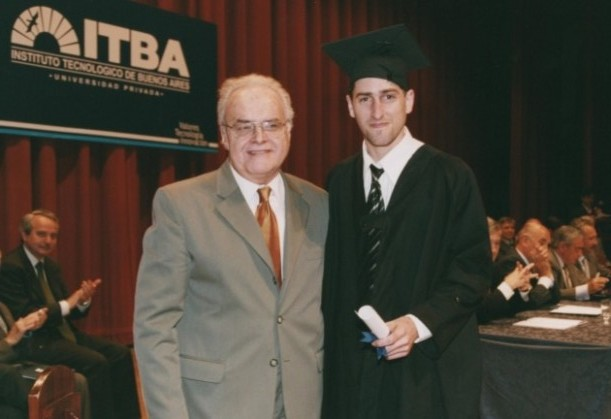
\includegraphics[width=\textwidth, frame]{foto_entrega_titulo.jpg}
            \caption{Diploma ceremony next profesor Eng. Eduardo Martinez.}
            \label{fig:foto_titulo}
         \end{subfigure} %
         \begin{subfigure}[b]{0.40\textwidth}
            \begin{center}
               
\includegraphics[width=0.6\textwidth, frame]{medalla_i+d_1.jpg}
               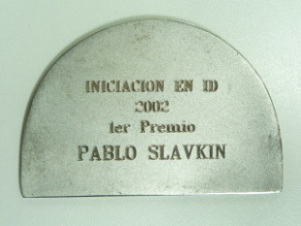
\includegraphics[width=0.6\textwidth, frame]{medalla_i+d_2.jpg}
               \caption{1\textsuperscript{th} prize medal in R\&D, research and development beginning, from ITBA university competition}
               \label{fig:medalla_i+d}
            \end{center}
         \end{subfigure}%
         \hfill
         \begin{subfigure}[b]{0.55\textwidth}
            
\includegraphics[width=\textwidth, frame]{robot.jpg}
            \caption{3\textsuperscript{th} prize on \emph{Battletek}, robot fight competition at ITBA university .}
            \label{fig:foto_robot}
         \end{subfigure}%
      \caption{Certificates and awards during engineering carer at ITBA university.}
      \label{fig:titulos_del_itba}
      \end{center}
   \end{figure}

   \begin{figure}
      \begin{center}
      \ContinuedFloat
         \begin{subfigure}[b]{0.40\textwidth}
            \begin{center}
               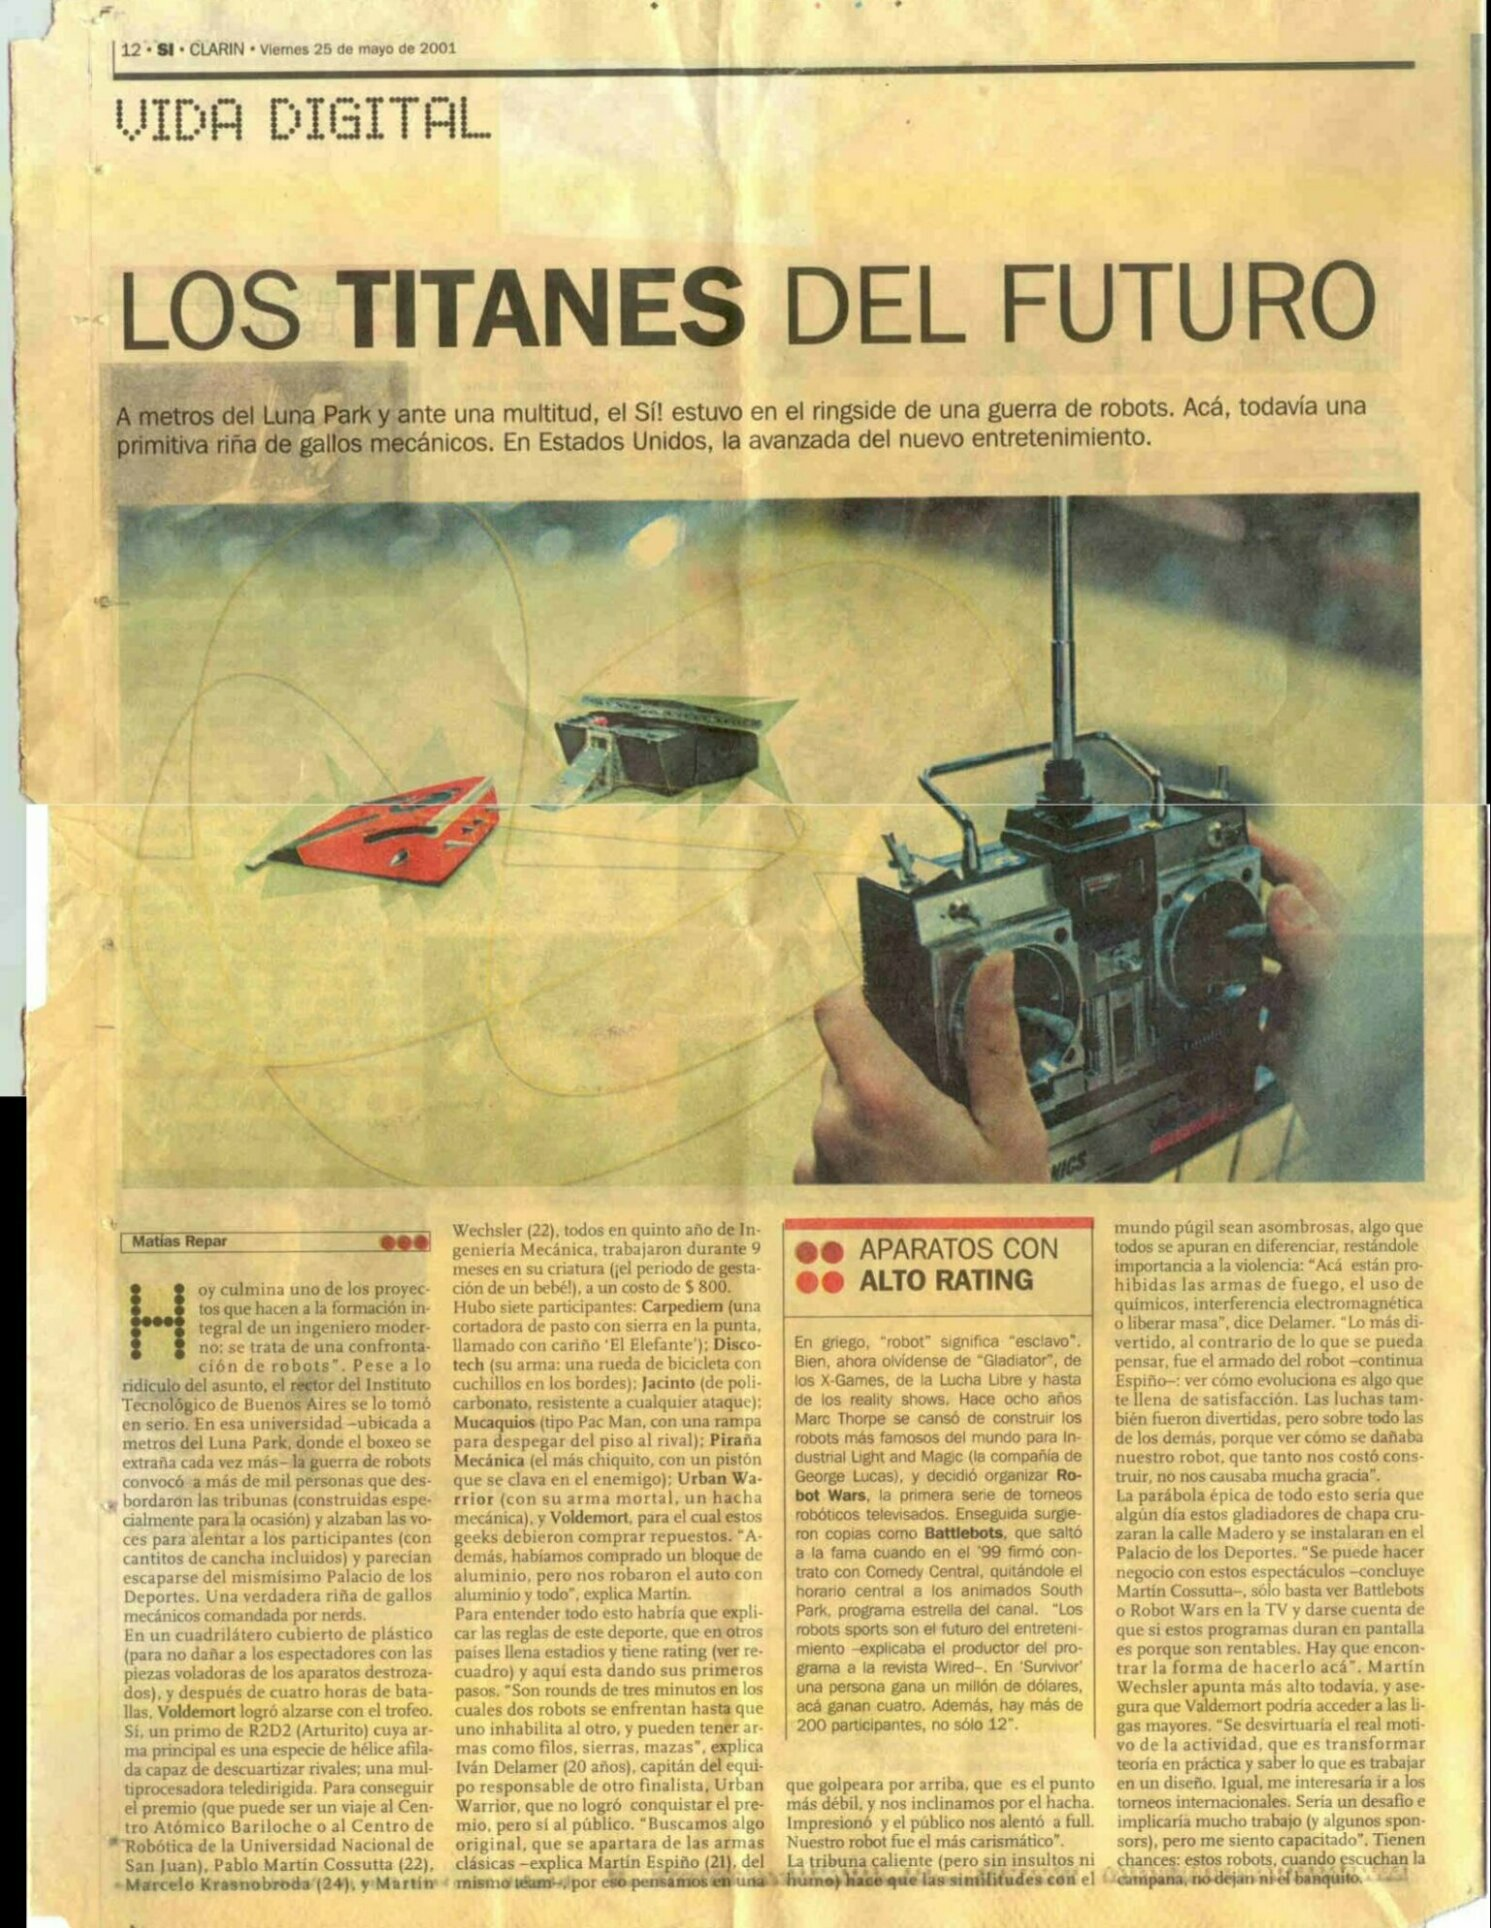
\includegraphics[width=\textwidth, frame]{robotdiario.jpg}
               \caption{Clarin newspaper note about robot fight competition participation. Black disco robot is from our team, called \emph{Discotech}}
               \label{fig:robotdiario}
            \end{center}
         \end{subfigure}%
         \hfill
         \begin{subfigure}[b]{0.55\textwidth}
            
\includegraphics[width=\textwidth, frame]{inteligencia_artificial.jpg}
            \caption{AI, artificial intelligence certificate at ITBA university course .}
            \label{fig:foto_ai}
         \end{subfigure}%
      \caption{Certificates and awards during engineering carer at ITBA university.}
      \label{fig:titulos_del_itba}
      \end{center}
   \end{figure}

   \begin{figure}
      \begin{center}
      \ContinuedFloat
         \begin{subfigure}[b]{0.45\textwidth}
            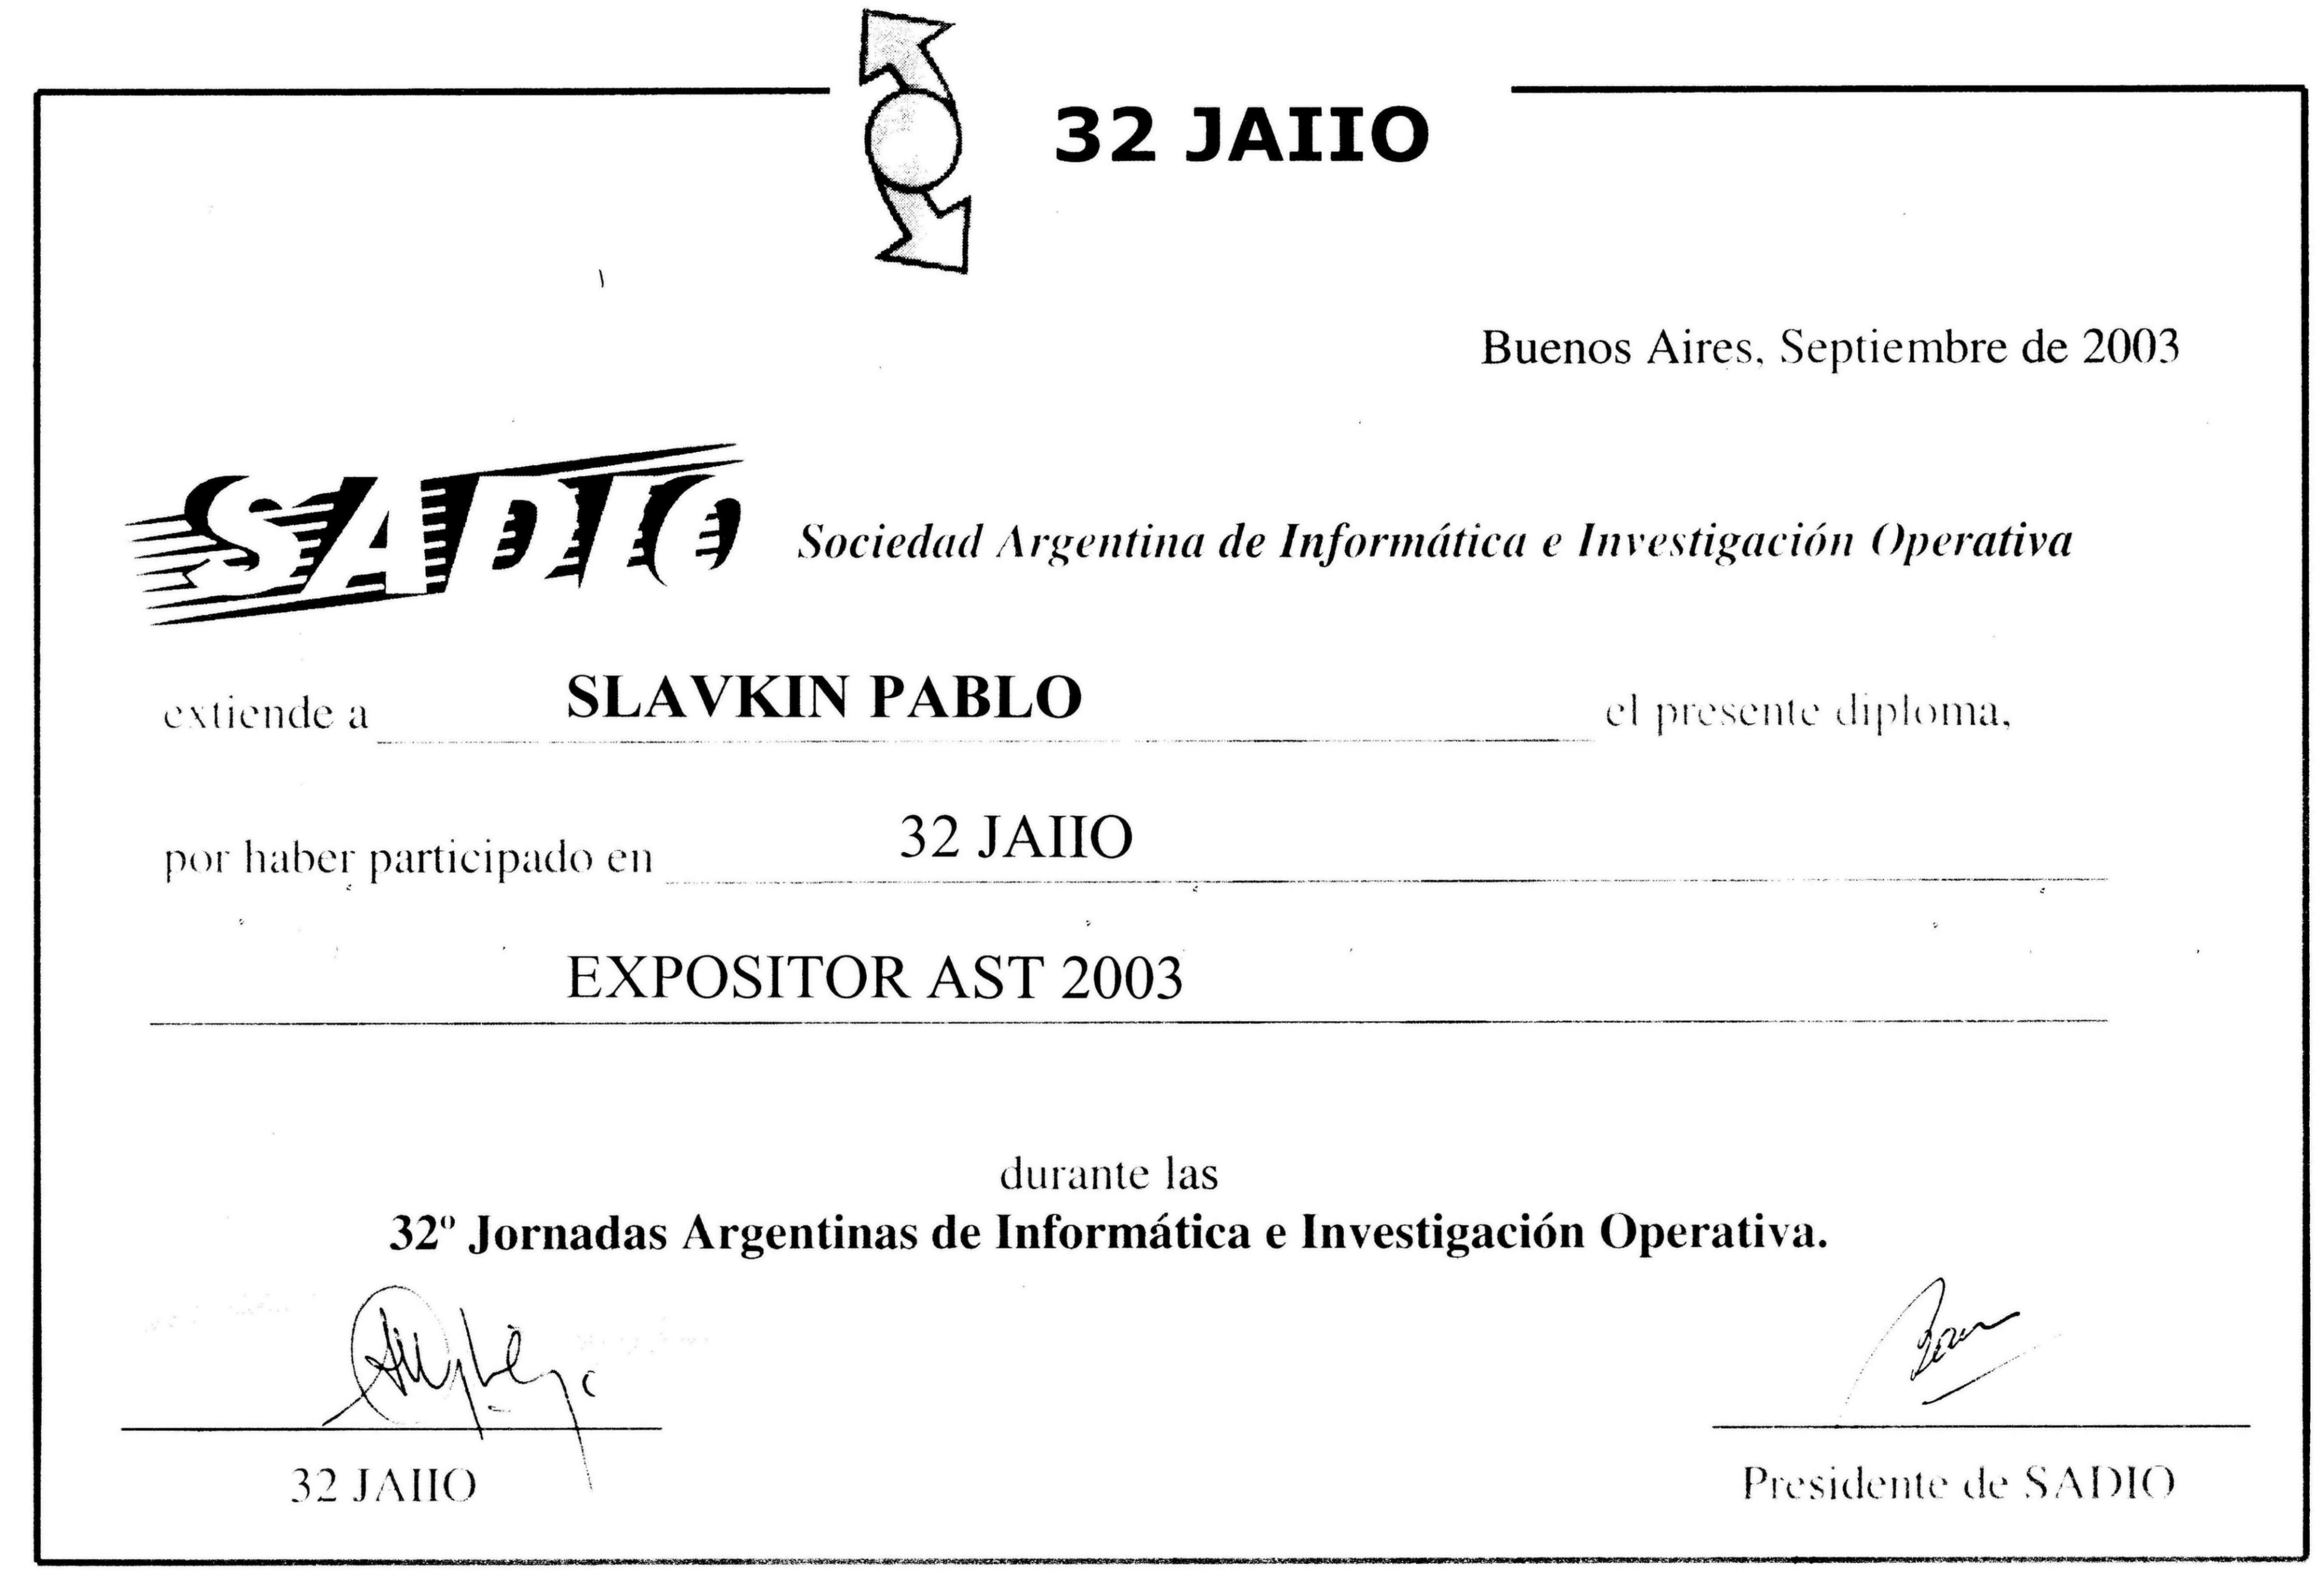
\includegraphics[width=\textwidth, frame]{sadio.jpg}
            \caption{JAIIO, 32\textsuperscript{o} Argentinian journals in Informatics and applied investigation at which we presented the paper \emph{Design and Simulation of a pipeline-structured Floating Point Unit for high performance general purpose processors.} \href \linkjaiio {read paper.}}
            \label{fig:jaiio}
         \end{subfigure}%
         \hfill
         \begin{subfigure}[b]{0.45\textwidth}
            
\includegraphics[width=\textwidth, frame]{cacic.jpg}
            \caption{CACIC, IX Argentinian Congress in Computer Science where we present the paper \emph{Selection of the Optimum Stage Number in Pipelined Floating-Point Units} \href \linkcacic {read paper.}}
            \label{fig:cacic}
         \end{subfigure}%
      \end{center}
      \caption{Certificates and awards during engineering carer at ITBA university.}
      \label{fig:titulos_del_itba}
   \end{figure}

   At figure \ref{fig:titulos_varios} there is certificates from mixed activities.
   \begin{figure}
      \begin{center}
         \begin{subfigure}[b]{0.45\textwidth}
            
\includegraphics[width=\textwidth, frame]{courses/cursolatex.pdf}
            \caption{{\LaTeX} introduction course certificate. Taken with the aim of profesional paper presentation and I work on {\LaTeX} every day since then.\href \linklatex {Ver certificado}}
            \label{fig:latex}
         \end{subfigure}%
         \hfill
         \begin{subfigure}[b]{0.45\textwidth}
            
\includegraphics[width=\textwidth, frame]{clase_robot_siglo21.jpg}
            \caption{Certificado por el dictado de un curso a escuela secundaria de introducción a la robótica, teórica y práctica. \href \linkrobotsiglo {Ver certificado}}
            \label{fig:robot_siglo_21}
         \end{subfigure}%

         \begin{subfigure}[b]{0.45\textwidth}
            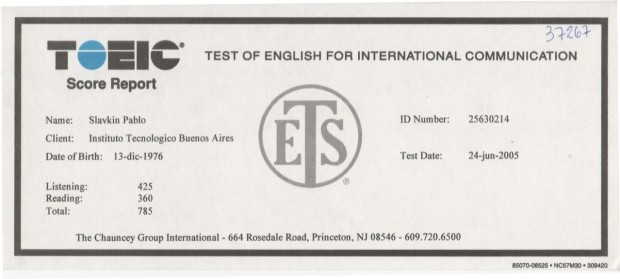
\includegraphics[width=\textwidth, frame]{courses/toeic.jpg}
            \caption{Certificado de examen de ingles TOEIC. \href \linktoeic {Ver certificado}}
            \label{fig:toeic}
         \end{subfigure}%
         \hfill
         \begin{subfigure}[b]{0.45\textwidth}
            
\includegraphics[width=\textwidth, frame]{courses/latam.pdf}
            \caption{Diploma de participacion en el concurso de proyectos LATAM 2018 organizado entre el MIT y el ITBA. \href \linklatam {Ver certificado} }
            \label{fig:latam}
         \end{subfigure}%
      \end{center}
      \caption{Certificados obtenidos en diferentes cursos y seminarios participando de manera independiente como parte de la actualización personal técnica y académica.}
      \label{fig:titulos_varios}
   \end{figure}

   At the figure \ref{fig:certificados_codility} there is some certificates and awards from Codility challenges platform that measure coding skills in different languages .
   \begin{figure}
      \begin{center}
         \begin{subfigure}[b]{0.45\textwidth}
            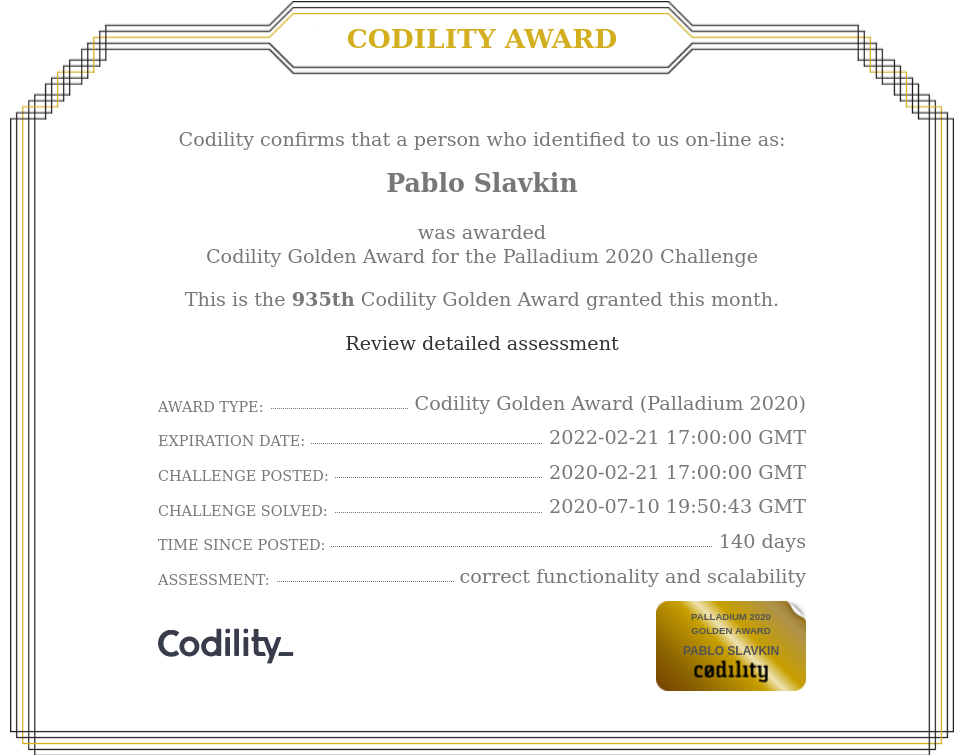
\includegraphics[width=\textwidth, frame]{codility_palladium_certificate.png}
            \caption{Golden award in Palladium challenge 2020 from Codility. Coded in C. \href {\linkcodilitycertone}{see certificate.}}
            \label{fig:latex}
         \end{subfigure}%
         \hfill
         \begin{subfigure}[b]{0.45\textwidth}
         \end{subfigure}%
      \end{center}

      \caption{Certificates from Codility platform}
      \label{fig:certificados_codility}
   \end{figure}
